\documentclass[notes,11pt, aspectratio=169]{beamer}

\usepackage{pgfpages}
% These slides also contain speaker notes. You can print just the slides,
% just the notes, or both, depending on the setting below. Comment out the want
% you want.
\setbeameroption{hide notes} % Only slide
%\setbeameroption{show only notes} % Only notes
%\setbeameroption{show notes on second screen=right} % Both

\usepackage{helvet}
\usepackage[default]{lato}
\usepackage{array}
\usepackage{tgbonum}

\usepackage{tikz}
\usepackage{verbatim}
\setbeamertemplate{note page}{\pagecolor{yellow!5}\insertnote}
\usetikzlibrary{positioning}
\usetikzlibrary{snakes}
\usetikzlibrary{calc}
\usetikzlibrary{arrows}
\usetikzlibrary{decorations.markings}
\usetikzlibrary{shapes.misc}
\usetikzlibrary{matrix,shapes,arrows,fit,tikzmark}
\usepackage{amsmath}
\usepackage{mathpazo}
\usepackage{hyperref}
\usepackage{lipsum}
\usepackage{multimedia}
\usepackage{graphicx}
\usepackage{multirow}
\usepackage{graphicx}
\usepackage{dcolumn}
\usepackage{bbm}
\newcolumntype{d}[0]{D{.}{.}{5}}

\usepackage{changepage}
\usepackage{appendixnumberbeamer}
\newcommand{\beginbackup}{
   \newcounter{framenumbervorappendix}
   \setcounter{framenumbervorappendix}{\value{framenumber}}
   \setbeamertemplate{footline}
   {
     \leavevmode%
     \hline
     box{%
       \begin{beamercolorbox}[wd=\paperwidth,ht=2.25ex,dp=1ex,right]{footlinecolor}%
%         \insertframenumber  \hspace*{2ex} 
       \end{beamercolorbox}}%
     \vskip0pt%
   }
 }
\newcommand{\backupend}{
   \addtocounter{framenumbervorappendix}{-\value{framenumber}}
   \addtocounter{framenumber}{\value{framenumbervorappendix}} 
}


\usepackage{graphicx}
\usepackage[space]{grffile}
\usepackage{booktabs}
\newcommand\independent{\protect\mathpalette{\protect\independenT}{\perp}}
\def\independenT#1#2{\mathrel{\rlap{$#1#2$}\mkern2mu{#1#2}}}
\DeclareMathOperator{\Supp}{Supp}


\newtheorem{assN}{Assumption}
% These are my colors -- there are many like them, but these ones are mine.
\definecolor{blue}{RGB}{0,114,178}
\definecolor{red}{RGB}{213,94,0}
\definecolor{yellow}{RGB}{240,228,66}
\definecolor{green}{RGB}{0,158,115}

\hypersetup{
  colorlinks=false,
  linkbordercolor = {white},
  linkcolor = {blue}
}


%% I use a beige off white for my background
\definecolor{MyBackground}{RGB}{255,253,218}

%% Uncomment this if you want to change the background color to something else
%\setbeamercolor{background canvas}{bg=MyBackground}

%% Change the bg color to adjust your transition slide background color!
\newenvironment{transitionframe}{
  \setbeamercolor{background canvas}{bg=yellow}
  \begin{frame}}{
    \end{frame}
}

\setbeamercolor{frametitle}{fg=blue}
\setbeamercolor{title}{fg=black}
\setbeamertemplate{footline}[frame number]
\setbeamertemplate{navigation symbols}{} 
\setbeamertemplate{itemize items}{-}
\setbeamercolor{itemize item}{fg=blue}
\setbeamercolor{itemize subitem}{fg=blue}
\setbeamercolor{enumerate item}{fg=blue}
\setbeamercolor{enumerate subitem}{fg=blue}
\setbeamercolor{button}{bg=MyBackground,fg=blue,}



% If you like road maps, rather than having clutter at the top, have a roadmap show up at the end of each section 
% (and after your introduction)
% Uncomment this is if you want the roadmap!
% \AtBeginSection[]
% {
%    \begin{frame}
%        \frametitle{Roadmap of Talk}
%        \tableofcontents[currentsection]
%    \end{frame}
% }
\setbeamercolor{section in toc}{fg=blue}
\setbeamercolor{subsection in toc}{fg=red}
\setbeamersize{text margin left=1em,text margin right=1em} 

\newenvironment{wideitemize}{\itemize\addtolength{\itemsep}{10pt}}{\enditemize}

\usepackage{environ}
\NewEnviron{videoframe}[1]{
  \begin{frame}
    \vspace{-8pt}
    \begin{columns}[onlytextwidth, T] % align columns
      \begin{column}{.70\textwidth}
        \begin{minipage}[t][\textheight][t]
          {\dimexpr\textwidth}
          \vspace{8pt}
          \hspace{4pt} {\Large \sc \textcolor{blue}{#1}}
          \vspace{8pt}
          
          \BODY
        \end{minipage}
      \end{column}%
      \hfill%
      \begin{column}{.38\textwidth}
        \colorbox{green!20}{\begin{minipage}[t][1.2\textheight][t]
            {\dimexpr\textwidth}
            Face goes here
          \end{minipage}}
      \end{column}%
    \end{columns}
  \end{frame}
}

\title[]{\textcolor{blue}{Canonical Research Designs V:\\ Bartik, Simulated, and Granular Instruments }}
\author[PGP]{}
\institute[FRBNY]{\small{\begin{tabular}{c}
  Paul Goldsmith-Pinkham  \\
\end{tabular}}}

\date{\today}

\begin{document}

%%% TIKZ STUFF
\tikzset{   
        every picture/.style={remember picture,baseline},
        every node/.style={anchor=base,align=center,outer sep=1.5pt},
        every path/.style={thick},
        }
\newcommand\marktopleft[1]{%
    \tikz[overlay,remember picture] 
        \node (marker-#1-a) at (-.3em,.3em) {};%
}
\newcommand\markbottomright[2]{%
    \tikz[overlay,remember picture] 
        \node (marker-#1-b) at (0em,0em) {};%
}
\tikzstyle{every picture}+=[remember picture] 
\tikzstyle{mybox} =[draw=black, very thick, rectangle, inner sep=10pt, inner ysep=20pt]
\tikzstyle{fancytitle} =[draw=black,fill=red, text=white]
%%%% END TIKZ STUFF

% Title Slide
\begin{frame}
\maketitle
\end{frame}

\begin{frame}{Roadmap for Today}
  \begin{wideitemize}
  \item In some cases, the source of exogeneous variation (either in an IV setting, or just OLS) is straightforward
    \begin{itemize}
    \item There is a single policy or source of variation
    \end{itemize}
  \item However, in other settings, there are more complicated sources of variation exploited to identify effects. Today we'll focus on three:
    \begin{itemize}
    \item Bartik (shift-share) instruments: three recent
      papers on commonly used identification approach
    \item Simulated instruments: reframe an older literature in a new
      light using Borusyak and Hull (2022) paper
    \item Granular instruments: identifcation approach in Gabaix and
      Koijen (2023) leveraging differences in the size distribution
      across firms
    \end{itemize}
  \item Key historical feature of some of these approaches is that
    they had an ``intuitive'' feature of identification, but formal
    properties were not established for several decades
    \begin{itemize}
    \item Analagous to staggered DinD lit!
    \end{itemize}
  \end{wideitemize}
\end{frame}

\section{Bartik Instruments}

\begin{frame}{Bartik instruments are used everywhere}
    %Local Markets and National Categories
  \begin{center}
    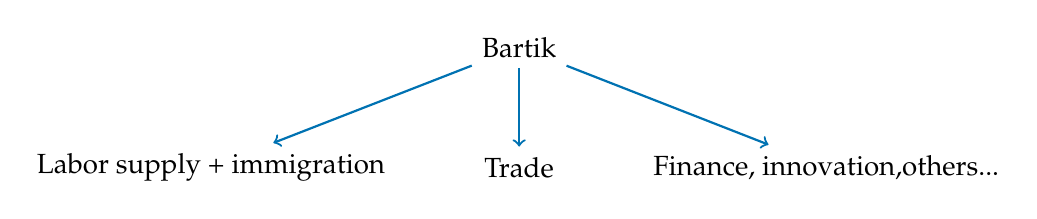
\begin{tikzpicture}[rectangle,draw=cyan,thick]
      \node (pq1) {Labor supply + immigration};
      \node [dashed,right=of pq1] (pq2) {Trade};
      \node [dashed,right=of pq2] (pq4) {Finance, innovation,\\ others...};
      \node [dashed,above=of pq2] (bartik) {Bartik};
      \path[->,thick,blue] (bartik) edge  (pq1)
      (bartik) edge  (pq2)
      (bartik) edge  (pq4);
    \end{tikzpicture}
  \end{center}
  \begin{itemize}
  \item Thread that links all Bartik applications:
    \begin{itemize}
    \item local markets composed of many ``categories''
    \item need for identification
    \end{itemize}
    \smallskip
  \item Approach has been used since the early 90:
    \begin{itemize}
    \item sometimes called ``shift-share'' or ``industry mix'' instruments
    \end{itemize}
  \end{itemize}
\end{frame}

\begin{frame}{Examples of Bartik instruments in many subfields}
  \begin{description}
  \item[Immigration:] Altonji and Card (1991), Card (2001)
    \smallskip
  \item[Bank Lending:] Amiti and Weinstein (2018), Greenstone, Mas and Nguyen (2015)
    \smallskip    
  \item[Market Size + Demography:] Acemoglu and Linn (2004), Jaravel (2018)
    \smallskip    
  \item[Labor Supply Elasticity:] Blanchard and Katz (1992), \textbf{Bartik} (1991)
    \smallskip
  \item[Fiscal Multipliers:] Nakamura and Steinsson (2014)
    \smallskip    
  \item[Trade + Labor:] Autor, Dorn, and Hanson (2013), Autor, Dorn and Hanson (2018), etc. 
    \smallskip    
  \item[Foreign Aid:] Nunn and Qian (2014)
    \smallskip
  \item[Portfolio Allocation:] Calvet, Campbell, and Sodini (2009)
    \smallskip
  \item[Trade + Prices:] Piveteau and Smagghue (2017), de Roux et al. (2017)
    \smallskip    
  \item[Automation:] Acemoglu and Restrepo (2017)
  \end{description}
\end{frame}

\begin{frame}{Many paths lead to Bartik}
  \begin{itemize}
  \item Diverse literature leads to many motivations and justifications for Bartik approach
    \medskip
  \item Two distinct approaches in the literature:
    \begin{enumerate}
    \item Applied micro statistical approach: interested in a reduced
      form causal relationship; need an instrument that is
      uncorrelated with error term; make argument that Bartik
      instrument is defensible \smallskip
    \item Structural approach: interested in particular parameters
      from model; assumptions of model motivate certain estimating
      equations
    \end{enumerate}
    \medskip
  \item So what is the Bartik approach anyway?
  \end{itemize}
\end{frame}


\begin{frame}
  \frametitle{Motivation: local labor market approaches + reduced form}

  Consider a local labor market regression like the following:  
  \begin{align}
    y_l &= \beta_0 + \beta x_l + \epsilon_l \notag 
  \end{align}

  \begin{itemize}
    \setlength\itemsep{1em}
  \item $\mathbb{E}[x_l\epsilon_l] \neq 0$   $\Rightarrow$ need an instrument to estimate $\beta$ 
  \item E.g. Autor, Dorn and Hanson (2013) setting:
    \begin{itemize}
      \setlength\itemsep{1em}
    \item $l$: location (commuting zone)
    \item $y_l$: manufacturing employment \textit{growth}
    \item  $x_l$: import exposure to China \textit{growth}
    \item $\beta$: effect of rise of China on manufacturing employment
    \item an instrument for location-level exposure to trade with China
    \end{itemize}
\end{itemize}


\end{frame}


%------------
\begin{frame}
\frametitle{The Bartik instrument}

Accounting identity \#1:
\begin{align}
  x_l &=  \sum_{k=1}^{K} z_{lk} g_{lk} \notag  
\end{align}
\begin{itemize}
\setlength\itemsep{1em}
  \item $z_{lk}$: location-industry shares  ($Z_l$)
  \item $g_{lk} $: location-industry growth (in imports) rates ($G_l$) 
  \end{itemize}
Accounting identity \#2:

$$\underbrace{ g_{lk}}_{\text{location-industry}} = \underbrace{  \textcolor{blue}{g}_{ \textcolor{blue}{k}}}_{\text{industry}} + \underbrace{  \textcolor{red}{\tilde{g}_{lk}}   }_{\substack{\text{idiosyncratic} \\ \text{location- industry}}} $$ 

Infeasible Bartik:
$$B_l = \sum_{k=1}^{K}z_{lk} \textcolor{blue}{g_{k}}$$

\end{frame}


%------
\begin{frame}
\frametitle{This gives us a simple 2SLS structure}


\begin{align}
  y_l&= \beta_0 + \beta x_l + \epsilon_l \notag \\
  x_l&= \pi_0 + \pi_{1} B_l + u_l \notag \\  
B_l &=  \sum_{k=1}^{K}z_{lk} \textcolor{blue}{g_{k}} \notag \\
g_{lk} &=   \textcolor{blue}{g}_{ \textcolor{blue}{k}}+  \textcolor{red}{\tilde{g}_{lk}}  \notag 
\end{align}

Bank-lending relationships: e.g., Greenstone, Mas and Nguyen (2015)
\begin{itemize}
\item $z_{lk}$: location (l) share of loan origination from bank $k$
\item $g_{lk}$:  loan growth in location $l$ by bank $k$
\item $\textcolor{blue}{g_k}$: part of loan growth due to bank supply shock
\end{itemize}


\end{frame}


%%%%%


\begin{frame}
\addtocounter{framenumber}{-1}
\frametitle{Other instruments have this structure}

\begin{align}
  y_l&= \beta_0 + \beta x_l + \epsilon_l \notag \\
  x_l&= \pi_0 + \pi_{1} B_l + u_l \notag \\  
B_l &=  \sum_{k=1}^{K}z_{lk} \textcolor{blue}{g_{k}} \notag \\
g_{lk} &=   \textcolor{blue}{g}_{ \textcolor{blue}{k}}+  \textcolor{red}{\tilde{g}_{lk}}  \notag 
\end{align}

Immigrant enclave: e.g., Altonji and Card (1991)
\begin{itemize}
\item $z_{lk}$: share of people from foreign $k$ living in $l$ (in a base period)
\item $g_{lk}$:  growth in number of people from $k$ to $l$
\item $\textcolor{blue}{g_k}$: growth in people from $k$ nationally
\end{itemize}


\end{frame}


%------
\begin{frame}
\addtocounter{framenumber}{-1}
\frametitle{Other instruments have this structure}

\begin{align}
  y_l&= \beta_0 + \beta x_l + \epsilon_l \notag \\
  x_l&= \pi_0 + \pi_{1} B_l + u_l \notag \\  
B_l &=  \sum_{k=1}^{K}z_{lk} \textcolor{blue}{g_{k}} \notag \\
g_{lk} &=   \textcolor{blue}{g}_{ \textcolor{blue}{k}}+  \textcolor{red}{\tilde{g}_{lk}}  \notag 
\end{align}

Market size and demography: e.g., Acemoglu and Linn (2004)
\begin{itemize}
\item $z_{lk}$: spending share on drug $l$ from age group $k$
\item $g_{lk}$:  growth in spending of group $k$ on drug $l$
\item $\textcolor{blue}{g_k}$: growth in spending of group $k$ (due to population aging)
\end{itemize}


\end{frame}

\begin{frame}
\frametitle{What's necessary for consistency?}

\begin{align}
  y_l&= \beta_0 + \beta x_l + \epsilon_l \notag \\
  x_l&= \pi_0 + \pi_{1} B_l + u_l \notag \\  
  B_l &=  \sum_{k=1}^{K}z_{lk} \textcolor{blue}{g_{k}} \notag \\
  g_{lk} &=   \textcolor{blue}{g}_{ \textcolor{blue}{k}}+  \textcolor{red}{\tilde{g}_{lk}}  \notag 
\end{align}

\begin{itemize}
\item We need $B_{l}$ to be a valid instrument
\item Requires two conditions with constant effects:
  \begin{enumerate}
  \item Relevance: $\pi_{1} \not=0$, e.g. $Cov(B_{l}, x_{l}) \not= 0$
  \item Exclusion: $E(B_{l}\epsilon_{l}) = 0$
  \end{enumerate}
\item Key flaw in this literature until recently: economic +
  statistical content of exclusion has been vague and sometimes confused
\end{itemize}

\end{frame}

\begin{frame}{Key thing to remember from today}
  \begin{itemize}
  \item Assuming independence or exogeneity on the basis of a model
    does not necessarily make it true
    \begin{itemize}
    \item E.g. Hausman instruments in IO models -- model may assume
      that exclusion restriction is satisfied, but not necessarily
      true in reality
    \end{itemize}
  \item Assuming that two things are independent because they don't
    seem ``related'' doesn't make it true 
    \begin{itemize}
    \item Bartik literature many times argues that national nature of
      shocks ``decouples'' the instrument from local market
      conditions. However, it still exploits local
      characteristics. Need to make very specific arguments to
      validate claim (will come to this).
    \end{itemize}
  \item When evaluating an identification strategy, you should be able
    to describe counterfactual claims using the measure. This is
    typically not concrete in Bartik -- try to make it concrete!
    What is exactly changing in China? Why is it random? 
  \end{itemize}
\end{frame}



%-----
\begin{frame}
\frametitle{More general econometric set-up}
\begin{align}
y_{lt} & =\mathbf{D}_{lt}\beta_0 +x_{lt}\beta+\epsilon_{lt}, \notag \\
x_{lt} & =\mathbf{D}_{lt}\tau+ B_{lt}\gamma+\eta_{lt}\notag \\
\mathbf{D}_{lt} &= \text{\footnotesize{controls, f.e.}} \notag \\
g_{lkt} &=   \textcolor{blue}{g_{ kt}} + \textcolor{red}{\tilde{g}_{lkt}}  \notag \\
B_{lt} &= \sum_{k=1}^K z_{lk0} \textcolor{blue}{g_{kt}}, \notag \\
\{\{  &  x_{lt},\mathbf{D}_{lt},\epsilon_{lt} \}_{t=1}^T\}_{l=1}^L, \text{ iid, } L\rightarrow \infty \notag
\end{align}



  Assumptions for IV in terms of $B_{lt}$:
  \begin{itemize}
	\setlength\itemsep{1em}
  \item Exogeneity: $\mathbb{E}\left[B_{lt}\epsilon_{lt}\middle| \mathbf{D}_{lt}\right] = 0$
  \item Relevance: $\text{Cov}\left[B_{lt}, x_{lt} \middle| \mathbf{D}_{lt}\right] \not= 0$
  \end{itemize}
  
    Question:
  \begin{itemize}
  \item What do these statements about $B_{lt}$ imply about $z_{lk0}$ and $\textcolor{blue}{g_{kt}}$?
%\item Vice-versa?
  \end{itemize}

\end{frame}

\begin{frame}{Recent Literature on this topic}
  \begin{wideitemize}
  \item Three papers addressed this question, and can be split into two grouping
  \item The division between papers can be split based on focus on $z_{lk0}$ vs. $g_{kt}$
    \begin{enumerate}
    \item Goldsmith-Pinkham, Sorkin and Swift (2020) focus on $z_{lk0}$ and make an analogy to difference-in-differences
    \item Adao, Kolesar and Morales (2019) and Borusyak, Hull and Jaravel (2020) focus on $g_{kt}$, and make a strong connection to the design based approach (e.g. these are as-if random shocks)
    \end{enumerate}
  \item Key problem, historically, in this literature, was the lack
    of a coherent defense of the identifying variation
    \begin{itemize}
      \item These papers provide a way of doing this! But you have to pick one approach
    \end{itemize}
  \end{wideitemize}
\end{frame}


%----
\begin{frame}
\frametitle{Understanding the identifying assumption in GPSS: Three  special cases}

\begin{enumerate}
  \setlength\itemsep{1em}
\item One time period, two industries
\item T time periods, two industries
\item One time period, K industries
\end{enumerate}

\end{frame}



%------
\begin{frame}[label=twoindustries]
\frametitle{Special case \#1: One time period, two industries}
\begin{itemize}
	\setlength\itemsep{1em}
\item $z_{l2}= 1-z_{l1}$ 
\item Bartik:  \begin{align*}B_l &= z_{l1} \textcolor{blue}{g_1} + z_{l2} \textcolor{blue}{g_2}  =z_{l1} \textcolor{blue}{g_1} + (1-z_{l1}) \textcolor{blue}{g_2} \notag \\
&=\textcolor{blue}{g_2}+ (\textcolor{blue}{g_1} - \textcolor{blue}{g_2}) z_{l1} \notag
\end{align*}
\end{itemize} 
First-stage:
\begin{align*}
x_l &= \gamma_0 + \gamma B_l + \eta_l \notag \\
%x_l &= \gamma_0 + \gamma (\hat{g}_2+ (\hat{g}_1 - \hat{g}_2) z_{l1}) + \eta_l \notag \\
x_l &= \underbrace{\gamma_0+\gamma \textcolor{blue}{g_2}}_{\text{constant}} + \underbrace{\gamma (\textcolor{blue}{g_1} - \textcolor{blue}{g_2})}_{\text{coefficient}} z_{l1} + \eta_l \notag 
\end{align*}

The instrument is $z_{l1}$, while $\textcolor{blue}{g_k}$ affects relevance

\hyperlink{whyolsisbiased}{\beamergotobutton{Why OLS is biased}}




\end{frame}










%---------
\begin{frame}
\frametitle{Special case \#2:  T time periods, two industries }



Panel Bartik:

$$B_{lt} = z_{l10} \textcolor{blue}{g_{1t}}  +z_{l20} \textcolor{blue}{g_{2t}} = \textcolor{blue}{g_{2t}} + \underbrace{ \textcolor{blue}{\Delta_{gt}}}_{g_{1t}-g_{2t}} z_{l10}$$




First stage:
\begin{align}
x_{lt} & =\tau_{l}+\tau_{t}+ \gamma B_{lt} +\eta_{lt} \notag\\
x_{lt} & =\tau_{l}+\underbrace{(\tau_{t}+\gamma \textcolor{blue}{g_{2t}})}_{\tilde{\tau_{t}}}+\underbrace{\gamma  \textcolor{blue}{\Delta_{gt}}}_{\tilde{\gamma}_{t}}z_{l10}+\eta_{lt} \notag
\end{align}




\begin{itemize}
\item Industry shares times time period is the instrument
\item (Updated industry shares: similar)
\end{itemize}


\end{frame}



%---------
\begin{frame}
\frametitle{Special case \#2:  T time periods, two industries }

\begin{itemize}
	\setlength\itemsep{1em}
\item Analogy to continuous difference-in-differences 
	\begin{itemize}
	\setlength\itemsep{1em}
	\item $\textcolor{blue}{\Delta_{gt}}$ is size of policy 
	\item $z_{l10}$ is exposure to policy
	\end{itemize} 
\item Sometimes a ``pre-period'' before policy: test for parallel pre-trends 
	\begin{itemize}
	\setlength\itemsep{1em}
	\item E.g., in ADH, what happens from 1970 to 1990?
	\end{itemize}
\end{itemize}
\end{frame}


%----
\begin{frame}[label=kindustries]
\frametitle{Special case \#3: One time period, K industries}

\begin{itemize}
	\setlength\itemsep{1em}
\item $\textcolor{blue}{G}$: $K \times 1$ vector of $\textcolor{blue}{g_k}$
\item $Z$: $L \times K$, matrix of $Z_l$
\item $Y^\perp$, $X^\perp$, $B = (Z \textcolor{blue}{G})$: $L \times 1$, vectors of $y_l^\perp$, $x_l^\perp$ and $B_l$
\item $\Omega$: $K\times K$
\end{itemize}



\begin{align*}
  \hat{\beta}_{Bartik} &= \frac{B^\prime  Y^\perp}{B^\prime X^\perp}\\
  \hat{\beta}_{GMM} &= \frac{(X^{\perp \prime}Z)\Omega (Z'Y^\perp)}{(X^{\perp \prime} Z)\Omega (Z'X^\perp)}
\end{align*} 

 If $\Omega = (\textcolor{blue}{G} \textcolor{blue}{G}^\prime)$, then $\hat{\beta}_{Bartik}=\hat{\beta}_{GMM}$   

\end{frame}

%-----
\begin{frame}
\frametitle{Full general result with $T$ time periods and $K$ industries}

Two estimators are numerically identical:
\begin{itemize}
\item TSLS with Bartik instrument
\item GMM with industry shares $\times$ time period as instruments and a particular weight matrix 
\end{itemize}
\begin{align*}
  \hat{\beta}_{Bartik} &= \frac{\mathbf{B}^\prime  \widetilde{\mathbf{Y}}^\perp}{\mathbf{B}^\prime \widetilde{\mathbf{X}}^\perp}\\
  \hat{\beta}_{GMM} &= \frac{(\mathbf{X}^{\perp \prime}\widetilde{\mathbf{Z}})\Omega (\widetilde{\mathbf{Z}}'\mathbf{Y}^\perp)}{(\mathbf{X}^{\perp \prime} \widetilde{\mathbf{Z}})\Omega (\widetilde{\mathbf{Z}}'\mathbf{X}^\perp)}
\end{align*} 
$\Omega = (\textcolor{blue}{\mathbf{G}}
\textcolor{blue}{\mathbf{G}}^\prime)$, and $\widetilde{\mathbf{Z}}$ is
an $LT \times KT$ stacked vector of $Z_{0}$ interacted with time fixed
effects and $\textcolor{blue}{\mathbf{G}}$ is a $KT \times 1$ stacked
vector of growth rates $g_{kt}$.

\end{frame}



%----
\begin{frame}
\frametitle{When is the estimator consistent for the estimand of interest?}
\begin{center}
\textbf{What is the identification condition?}
\end{center}

$$\hat{\beta}_{Bartik}=  \frac{  \sum_{l=1}^L \sum_{t=1}^T \sum_{k=1}^K  z_{lkt} \textcolor{blue}{g_{kt}} y_{lt}^\perp    }{   \sum_{l=1}^L \sum_{t=1}^T \sum_{k=1}^K  z_{lkt} \textcolor{blue}{g_{kt}} x_{lt}^\perp   }  $$

Two ideas:
\begin{itemize}
\item ``Shares'' : talk about properties of $z_{lkt}$
	\begin{itemize}
	\item Conditional exogeneity
        \item \emph{model based} -- diff-in-diff style approach
	\end{itemize}
\item ``Shocks'' (Borusyak, Hull and Jaravel (2018)): talk about properties of $g_{kt}$
	\begin{itemize}
	\item Random, and a large number (equivalent industry-level regression)
        \item \emph{design-based} (in spirit) -- IV strategy
	\end{itemize}
\end{itemize}

\end{frame}

%----
%----
\begin{frame}
\frametitle{When are these views plausible? What do they mean?}


\textbf{Shares}

\textit{Conditional} exogeneity:
\begin{itemize}
\item Typically: exogenous to changes in error term, not levels of outcome
\item Standard in diff-in-diff (exclusion): in a period, exposure to an industry matters for outcome only through $x$
\end{itemize}


\textbf{Shocks}

\begin{itemize}
\item Large number of industries (shares are misspecified, need it to average out)
\item Random shocks across industries -- need the shocks to be conditionally random
\end{itemize}


\textbf{How do we choose?}
\begin{itemize}
\item The shocks approach is more design-based (which can be
  appealing), but requires an argument why shocks are randomly
  assigned
\item The shares approach is model-based, so suffers from same issues
  as diff-in-diff, but may more naturally work in your setting.
\end{itemize}

\end{frame}

%----
\begin{frame}
\frametitle{How to decide if a paper is  about shocks or shares?}

For Autor, Dorn and Hanson's China Shock:
Shocks:
\begin{itemize}
\item  Explains why $g_{kt}^{high-income}$ rather than $g_{kt}^{US}$  (hard to rationalize under shares)
\item Natural in a trade model: why would imports from China rise (in a trade model)?  Independent industry-specific shocks
\end{itemize}

Shares:
\begin{itemize}
\item Explains why $z_{lkt-1}$ rather than $z_{lkt}$ (hard to rationalize under shocks)
\item Explains why it is important for identification to study local labor markets (as opposed to parameter of interest where we want to think about spillovers)
\end{itemize}

\medskip

Bottom line: a little hard to tell what exactly ADH are assuming; ADH approach does not appear to satisfy testable assumptions under GPSS, but do appear to under BHJ.
\end{frame}








%%---
\begin{frame}[label=rotemberg]
\frametitle{Decomposing Bartik (GPSS 2020)}
\begin{center}
(Special case of Rotemberg (1983), proposition 1)
\end{center}
\vspace{0.2in}




$$\hat{\beta}_{Bartik} =\sum_k  \hat{\alpha}_k \hat{\beta}_k , \text{      } \sum_k \hat{\alpha}_k=1$$   
IV estimate using only the $k^{th}$ instrument:
$$\hat{\beta}_k = (Z_k^\prime X)^{-1} Z_k^\prime Y$$
``Rotemberg'' weight:
$$ \hat{\alpha}_k = \frac{ \textcolor{blue}{g_k} Z_k^\prime X}{\sum_{k=1}^K \textcolor{blue}{g_k} Z_k^\prime X}$$



\hyperlink{rotproof}{\beamergotobutton{Proof}}

\end{frame}




%----
\begin{frame}
\frametitle{Interpretation: sensitivity to misspecification elasticity}
\begin{center}
  Conley, Hansen and Rossi (2012); Andrews, Gentzkow and Shapiro (2017)\\
  Local misspecification:  $\epsilon_{lt} = L^{-1/2}V_{lt} + \tilde{\epsilon}_{lt}, \enskip Cov(V_{lt}, Z_{lt}) \not=0$,
\end{center}

\begin{itemize}
 \item $   \sqrt{L}\left(\hat{\beta} - \beta_0\right) \xrightarrow{\enskip d \enskip} \tilde{\beta}, \qquad \mathbb{E}\left[\tilde{\beta}\right] = \text{bias (misspecification) of Bartik instrument}$
 \item $   \sqrt{L}\left(\hat{\beta}_{k} - \beta_0\right) \xrightarrow{\enskip d \enskip} \tilde{\beta}_{k}, \qquad \mathbb{E}\left[\tilde{\beta}_{k}\right] = \text{bias (misspecification) of  $k$th  instrument}$

\end{itemize}

Suppose $\beta_0 \neq 0$.  Percentage bias:
\begin{equation}
  \frac{\mathbb{E}[\tilde{\beta}]}{\beta_{0}} = \sum_{k}\alpha_{k}\frac{\mathbb{E}[\tilde{\beta}_{k}]}{\beta_{0}} \notag
\end{equation} 
Industry with high $\alpha_k$: 
\begin{itemize}
\item an industry where it matters whether it is misspecified (endogenous) 
	\begin{itemize}
\item  because it is ``important'' in the estimate
	\end{itemize}
\end{itemize}


\end{frame}



%----
\begin{frame}[label=top5weights]
\textbf{Top five industries (out of 397)}



\begin{center}
\begin{tabular}{lllllllllllll}
\toprule
& $\hat{\alpha}_k$ & $g_k^{\text{high-income}}$ & $\hat{\beta}_k$  \\ \cmidrule(lr){2-4} 
Games and Toys & 0.182 & 174.841 & -0.151  \\  
Electronic Computers & 0.182 & 85.017 & -0.620  \\ 
Household Audio and Video & 0.130 & 118.879 & 0.287  \\ 
Computer Equipment & 0.076 & 28.110 & -0.315  \\ 
Telephone Apparatus & 0.058 & 37.454 & -0.305  \\ 
\bottomrule 
& \multicolumn{2}{l}{$0.628 \big/ 1.379$}   & -0.230 &\\
\end{tabular}
\end{center}
  
\footnotesize
\medskip
\begin{quote}
The \textbf{main source of variation in exposure is} within-manufacturing specialization in industries subject to different degrees of import competition...there is differentiation according to \textbf{local labor market reliance on labor-intensive industries}...By 2007, China accounted for over 40 percent of US imports in four four-digit SIC industries (\textbf{luggage, rubber and plastic footwear, games and toys, and die-cut paperboard}) and over 30 percent in 28 other industries, including \textbf{apparel, textiles, furniture, leather goods, electrical appliances, and jewelry}.
\end{quote}
\begin{center}
--- Autor, Dorn and Hanson (2013) , pg. 2123
\end{center}

\end{frame}


%----
\begin{frame}
\frametitle{Three tests of the identifying condition (under GPSS (2020)}

\begin{enumerate}
\item Confounds (or correlates)
\item Pre-trends 
\item Alternative estimators and overidentification
\end{enumerate}

\begin{wideitemize}
\item There are \emph{also} tests for BHJ -- similar to assuming
  strict ignorability, you can test for balance on observables
  (like the confounds above) of industries and locations
\end{wideitemize}

\end{frame}


%-----

\begin{frame}[label=overidtest]
\frametitle{Alternative estimators and overidentification tests}

Basic insight in GPSS: many instruments 
\begin{itemize}
\item Estimators (maximum likelihood): LIML, Hausman, Newey, Woutersen, Chao and Swanson (2012) HFUL (heteroskedasticity-Fuller (1977))
\item Estimators (two-step):  TSLS (problematic), Bartik TSLS, MBTSLS (Anatolyev (2013), and Kolesar et al (2015)) 
\end{itemize} 
Interpretation:
\begin{itemize}
\item Gap between maximum likelihood and two-step estimators is evidence of misspecification 
\end{itemize}
Also, overidentification tests, which provides evidence of misspecification (but not robust to heterogeneous effects!)

\end{frame}

% INTRO

\begin{frame}{Switching gears: Economists have a nose for randomness}
\begin{columns}[T] % align columns
\begin{column}{.5\textwidth}
  \begin{wideitemize}
  \item Paraphrasing a Yale prof:
    \begin{quote}
      Economists are really good at doing \emph{almost} the right
      thing in empirical work.\\
      \hfill -Anonymous Yale Professor
    \end{quote}
  \item Economists are clever at finding things that look convincingly
    ``random''
    \begin{itemize}
    \item Sometimes, it is easy to know how to use this randomness
    \end{itemize}
  \end{wideitemize}
\end{column}%
\hfill%
\begin{column}{.5\textwidth}
  \makebox[\linewidth][c]{
    \resizebox{\linewidth}{!}{
      
\includegraphics{images/twitter.png}
    }}
\end{column}%
\end{columns}
\end{frame}

\begin{frame}{Borusyak and Hull (2022) on exploiting randomness in IV}
\begin{columns}[T] % align columns
\begin{column}{.6\textwidth}
  \begin{wideitemize}
  \item Two key parts to this paper:
    \begin{enumerate}
    \item Highlighting how seemingly complicated \underline{research designs} can be framed as generalized propensity scores
    \item How complicated \underline{research designs} can suffer from \emph{interference} 
    \end{enumerate}
  \item There are many interesting results that spiral out from these
    two insights, but these are the key kernels (third piece is
    thinking about uncertainty using randomization inference, but deeply
    tied to other pieces))
  \item Will first start with showing how complicated research designs $\rightarrow$ propensity scores
  \end{wideitemize}
\end{column}%
\hfill%
\begin{column}{.38\textwidth}
  \makebox[\linewidth][c]{
    \resizebox{\linewidth}{!}{
      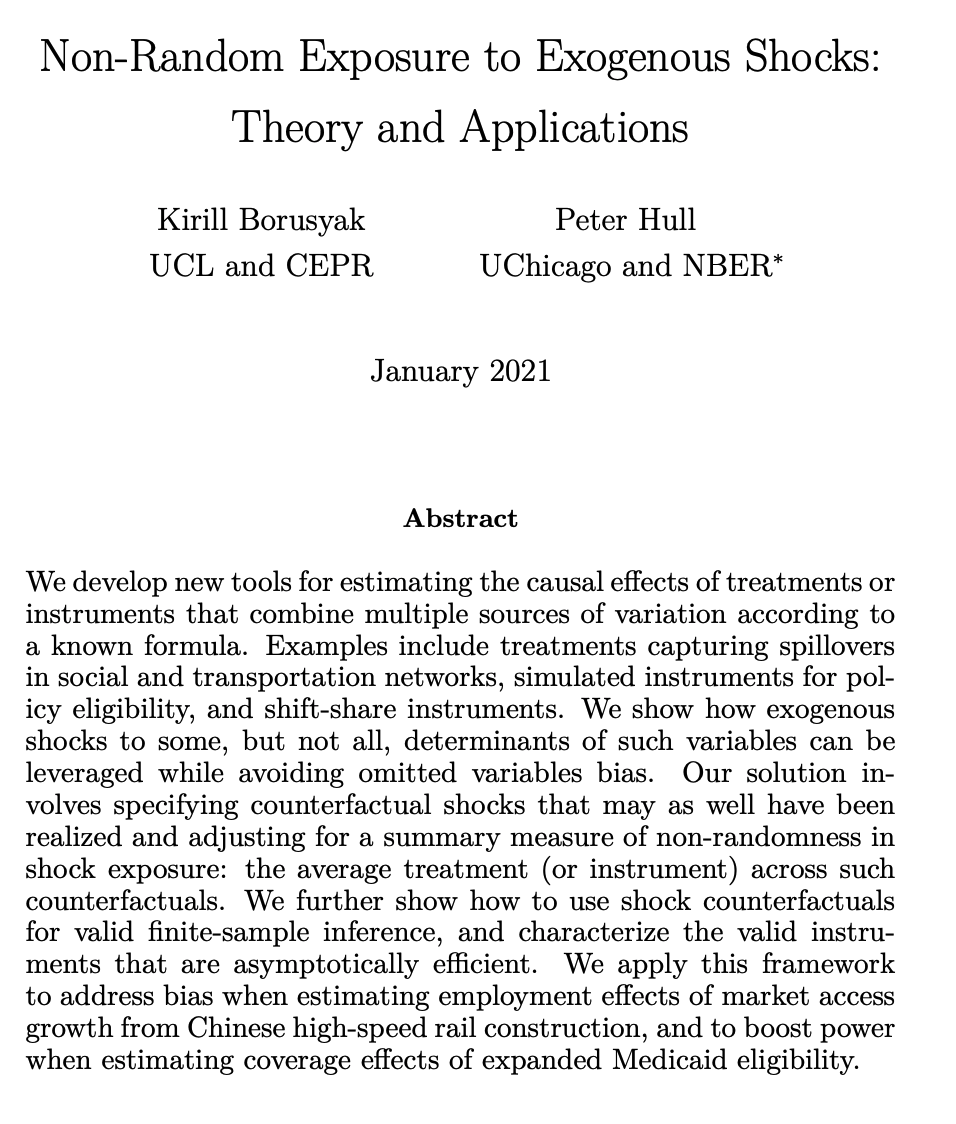
\includegraphics{images/abstract.png}
    }}
\end{column}%
\end{columns}
\end{frame}

\begin{frame}{Research designs from simple to complex}
\begin{columns}[T] % align columns
\begin{column}{.75\textwidth}
  \begin{wideitemize}
  \item Consider the trivial research design, following an RCT that
    randomly assigns $x_{i} \in \{0, 1\}$, and we want to estimate the
    effect of $x_{i}$ on $y_{i}$:
    \begin{equation*}
      y_{i} = \alpha + x_{i}\beta + \epsilon_{i}
    \end{equation*}
  \item The research design is effectively a coin flip:
    $E(x_{i}) = p$, and each $x_{i}$ is independent for each $i$
    \begin{itemize}
    \item $\beta$ is identified thanks to this coin flip design
    \end{itemize}
  \item This is true even when we have covariates, $w_{i}$ that stratify the experiment. We just need to control for $w_{i}$ correctly:  $E(x_{i}|w_{i}) = p(w_{i})$ and we can estimate the ATE directly
    % \begin{equation}
    %   \beta = \sum_{i} y_{i}x_{i}/p(w_{i}) -y_{i}(1-x_{i})/(1-p(w_{i}))
    % \end{equation}
  \item Effectively, the (potentially) endogenous $w_{i}$ affects
    treatment, but if we condition correctly, we can still identify a
    causal effect
  \end{wideitemize}
\end{column}%
\hfill%
\begin{column}{.25\textwidth}
  \makebox[\linewidth][c]{
    \resizebox{\linewidth}{!}{
      
\includegraphics{images/coinflip.jpeg}
    }}
\end{column}%
\end{columns}
\end{frame}


\begin{frame}{Research designs from simple to complex- Medicaid eligibility}
\begin{columns}[T] % align columns
\begin{column}{.75\textwidth}
  \begin{wideitemize}
  \item Now imagine the eligibility rules for Medicaid were being  randomly assigned
    \begin{itemize}
    \item Drawn from a bag just like marbles, completely randomly
    \end{itemize}
  \item We can now estimate the effect of Medicaid eligibility on things like child mortality
    \begin{itemize}
    \item Issue: eligibility is also a function of many \emph{endogenous} features
    \end{itemize}
    \item We consider a known
      function, $f_{i}$, and eligibility rules, $g_{i}$, such that
      $x_{i} = f(g_{i}, w_{i})$ maps the $w_{i}$ characteristics using
      the randomly drawn eligilibility rules
      \begin{itemize}
      \item Much like $w_{i}$ strata case, but more complex b/c can be high-dimensional / non-linear
      \end{itemize}
  \end{wideitemize}
\end{column}%
\hfill%
\begin{column}{.25\textwidth}
  \only<1>{  \makebox[\linewidth][c]{
    \resizebox{\linewidth}{!}{
      
\includegraphics{images/marbles.jpeg}
    }}}
\end{column}%
\end{columns}
\end{frame}

\begin{frame}{Simulated instruments as a  way to get a handle on this}
\begin{columns}[T] % align columns
\begin{column}{.5\textwidth}
  \begin{wideitemize}
  \item The challenge is that $g_{i}$ is a complicated variable -- it
    is a set of rules of that potentially complicated and hard to map
    to an ``instrument'' or ``treatment''
  \item You don't want to just use $x_{i}$ because it contains endogenous $w_{i}$
  \item Currie and Gruber (1996) solution: construct a variable
    $z_{i} = \sum_{j} f(g_{i}, w_{j})$ which takes $w$ from a random
    population (outside the state) and uses it to construct a
    ``predicted'' $x$
    \begin{itemize}
    \item Intuitively, hold fixed the $g_{i}$ and average over some
      distribution of $w_j$
    \end{itemize}
  \end{wideitemize}
\end{column}%
\hfill%
\begin{column}{.5\textwidth}
    \only<1>{  \makebox[\linewidth][c]{
    \resizebox{\linewidth}{!}{
      
\includegraphics{images/savingbabies.png}
    }}}
    \only<2>{  \makebox[\linewidth][c]{
    \resizebox{\linewidth}{!}{
      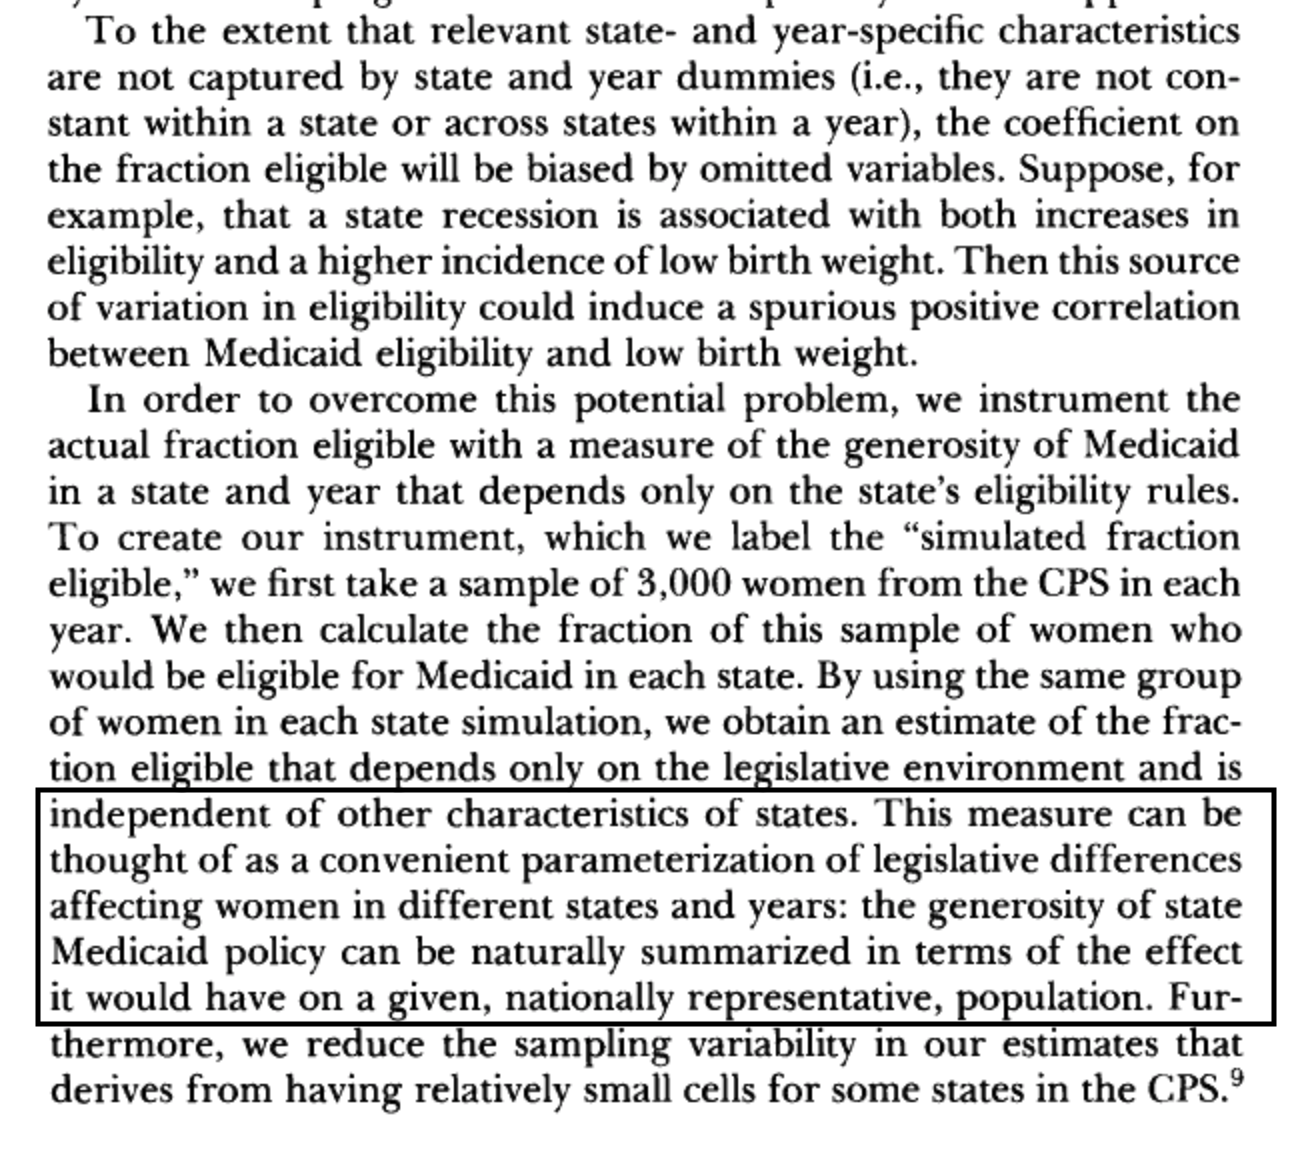
\includegraphics{images/savingbabies2.png}
    }}}
\end{column}%
\end{columns}
\end{frame}

\begin{frame}{This paper's approach vs. simulated instrument}
\begin{columns}[T] % align columns
\begin{column}{.9\textwidth}
  \begin{wideitemize}
  \item This is not the most efficient way to exploit this variation
  \item Remember our propensity score example: if we could just
    condition directly on $w_{i}$, then we would not worry about
    endogeneity
    \begin{itemize}
    \item The solution, then, is to construct a propensity score and condition on that!
    \end{itemize}
  \item Intuitively, ``the eligibility rules for Medicaid were being randomly assigned''
    \begin{itemize}
    \item In other words, we assert a counterfactual distribution over
      the policy rules $Pr(g)$
    \item This allows us to construct the propensity score for a given individual
    \end{itemize}
    \begin{equation*}
      p(w_{i}) = Pr(x_{i} | w_{i}) = \sum_{g} f_{i}(g, w_{i}) Pr(g)
    \end{equation*}
  \item With pscore in hand, estimation is straightforward, and known to be semiparametrically efficient!
    \begin{itemize}
    \item Either subtract this p-score off of the endogeneous variable
      (recentering) or control for it directly
    \end{itemize}
  \end{wideitemize}
\end{column}%
\hfill%
\begin{column}{.25\textwidth}
\end{column}%
\end{columns}
\end{frame}

\begin{frame}{The return on propensity scores in an empirical example}
  \begin{wideitemize}
  \item Medicaid Empirical example in this paper: ACA medicaid expansion
  \item ACA expanded Medicaid in only some states thanks to NFIB v. Seblius allowing choice by states
  \item Interested in understanding compositional shifts in health care across states
    \begin{itemize}
    \item Use ACS micro data and consider structural equation
      \begin{align*}
        y_{it} &= x_{it}\beta + \alpha_{s(i)} + \alpha_{t} + \epsilon_{it}
      \end{align*}
    \item $y_{it} $ are different health insurance take-up; $x_{it}$ is Medicaid eligibility for individual $i$
    \end{itemize}
  \item ``Simulated'' IV: dummy for whether state expanded Medicaid $z_{sim}$
  \item Borusyak and Hull IV: construct a person-level indicator for
    whether a person is eligible under their state's law $z_{bh}$
    \begin{itemize}
    \item Also identify the $p(w)$ that they are eligible on average across others states' laws
    \item They recenter ($\tilde{z}_{bh} = z_{bh} - p(w)$) 
    \end{itemize}
  \end{wideitemize}
\end{frame}

\begin{frame}{The return on propensity scores in an empirical example}
\begin{columns}[T] % align columns
\begin{column}{.25\textwidth}
  \begin{wideitemize}
  \item \textbf{Much} more precise
  \item Makes sense!
  \item Seems like we should use it...
  \end{wideitemize}
\end{column}%
\hfill%
\begin{column}{.8\textwidth}
    \makebox[\linewidth][c]{
    \resizebox{\linewidth}{!}{
      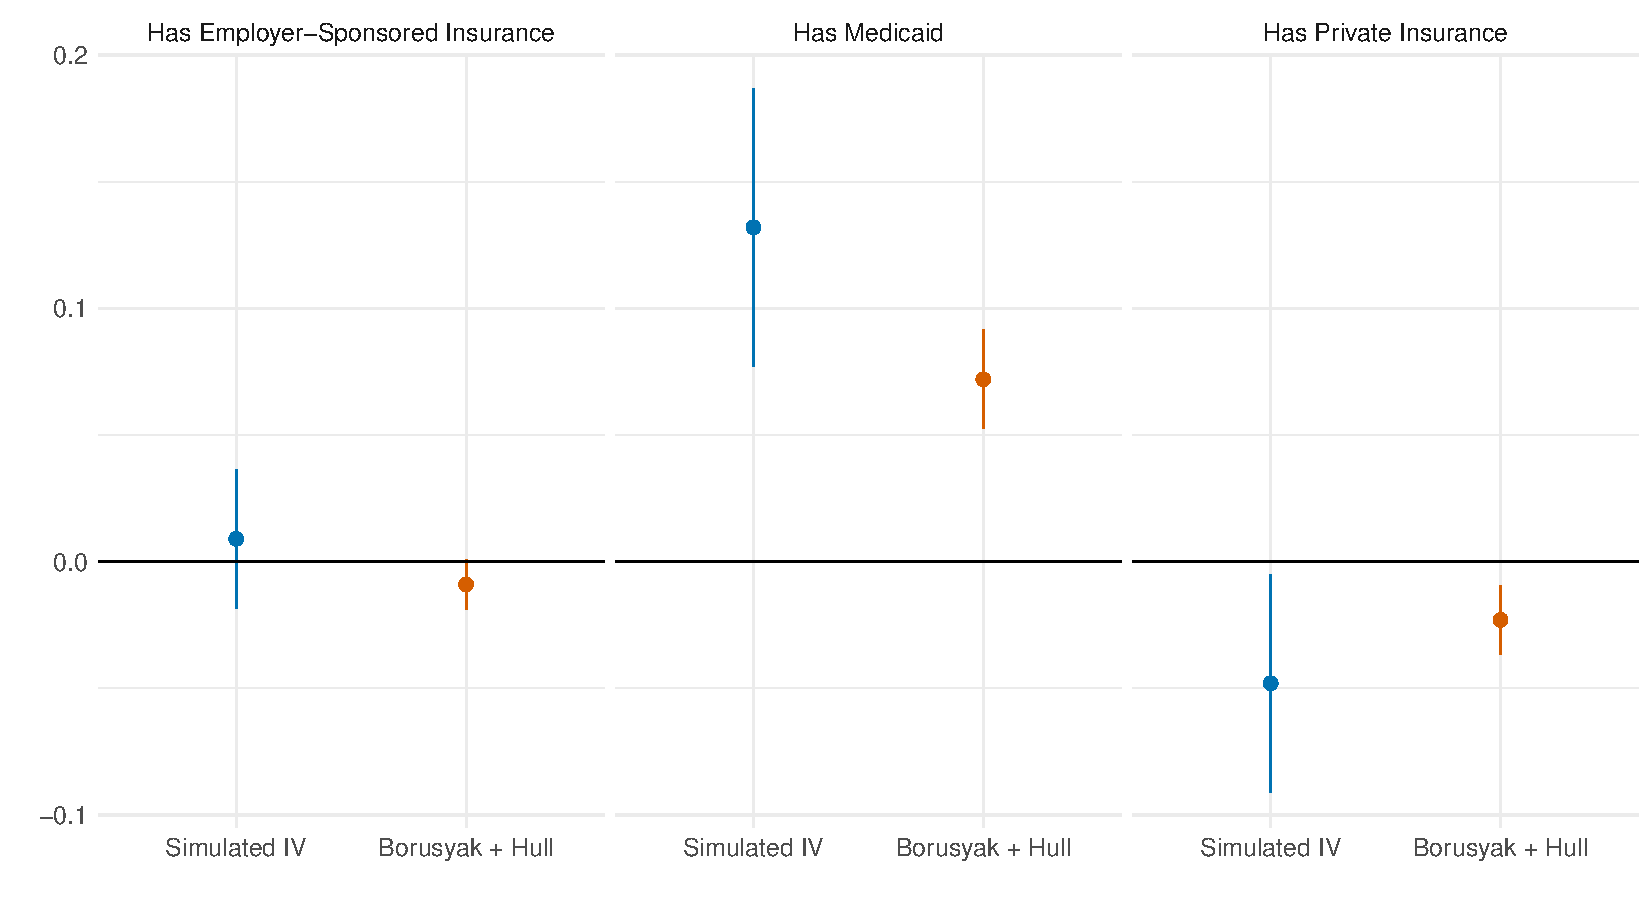
\includegraphics{images/medicaid.pdf}
    }}

\end{column}%
\end{columns}
\end{frame}

\begin{frame}{Second kernel of the paper: interference}
\begin{columns}[T] % align columns
\begin{column}{.75\textwidth}
  \begin{wideitemize}

  \item Medicaid example is simple to think about, and clarifies idea that:
    \begin{enumerate}
    \item Can convert high-dimensional variation into simple treatment effects
    \item Can be more \emph{efficient} (e.g. smaller s.e.) 
    \end{enumerate}
  \item However, you can take this much further.
  \item Consider the design of a railroad. Imagine the world in which
    a railroad designer randomly threw darts on a map to decide where
    to construct train lines
    \begin{itemize}
    \item Similar to the analogy of ``drawing'' the Medicaid
      eligibility rules
    \item But now, how do we think about the ``random'' piece
      interacting with different places?
    \item Let's start with something simple first
    \end{itemize}
  \end{wideitemize}
\end{column}%
\hfill%
\begin{column}{.25\textwidth}
    \only<1>{ \vfill \makebox[\linewidth][c]{
    \resizebox{\linewidth}{!}{
      \includegraphics{images/darts_map.jpeg}
    }}}
\end{column}%
\end{columns}
\end{frame}



\begin{frame}{ Interference in network settings }
\begin{columns}[T] % align columns
\begin{column}{.9\textwidth}
  \begin{wideitemize}
  \item Consider a setting where the researcher want to measure the impact of a
    randomized experiment on a network
    \begin{itemize}
    \item In other words, for a given person $i$, and observed network $W$, we randomly treat some subset of individuals on the network.
    \item We want to know what the effect of having more treated
      individuals connected to you $x_{i}$ is on $y_{i}$
    \end{itemize}
  \item Insight from paper: since the position in \emph{network} affects probability of being connected to individuals, some individuals will inherently get more exposure!
    \begin{itemize}
    \item Analogous to the friendship paradox
    \end{itemize}
  \item Need to construct an analogous propensity score for the
    network setting, and control for that
    \begin{itemize}
    \item Since we have a true RCT, this is not too hard!
    \item (But we do have to make decisions about what the spillover is)
    \item Aronow and Samii (2017) made serious progress on the network
      context
    \end{itemize}
  \end{wideitemize}
\end{column}%
\hfill%
\begin{column}{.45\textwidth}
    % \only<1>{  \makebox[\linewidth][c]{
    % \resizebox{\linewidth}{!}{
    %   \includegraphics{darts_map.jpeg}
    % }}}
\end{column}%
\end{columns}
\end{frame}


\begin{frame}{ Interference in spatial settings}
\begin{columns}[T] % align columns
\begin{column}{.95\textwidth}
  \begin{wideitemize}
  \item Things can be more confusing than an RCT, but this same insight applies
    \begin{itemize}
    \item Even with random shocks (darts on a board), some locations / people attract more treatment than others
    \item Consider the application from the paper
    \end{itemize}
  \item Estimate the impact of market access growth ($MA$) on land values growth ($V$) in China
    \begin{itemize}
    \item $MA$ is influenced by transportation networks, and measures aggregated access to other populations
      \begin{equation*}
        MA_{it} = \sum_{j}\tau(\mathbf{g}_{t}, loc_{i}, loc_{j})^{-1}pop_{j}
      \end{equation*}
    \end{itemize}
  \item Want to estimate the effect of $MA_{it}$ using ``random'' variation in network changes!
    \begin{itemize}
    \item Can we just run the OLS? No!
    \end{itemize}
  \end{wideitemize}
\end{column}%
\hfill%
\begin{column}{.45\textwidth}
    % \only<1>{  \makebox[\linewidth][c]{
    % \resizebox{\linewidth}{!}{
    %   \includegraphics{darts_map.jpeg}
    % }}}
\end{column}%
\end{columns}
\end{frame}

\begin{frame}{ Stylized Example of Market Access on a Square Island}
\begin{columns}[T] % align columns
\begin{column}{.55\textwidth}
  \begin{wideitemize}
  \item Take a square with square villages and randomly assign roads
  \item How does market access change?
  \item<2-> If we rerandomize, does it look different?
  \item<3-> As with the network, some places get more market access than others on average!
    \item<3-> Need to account for this propensity difference
  \end{wideitemize}
\end{column}%
\hfill%
\begin{column}{.45\textwidth}
    \only<1>{  \makebox[\linewidth][c]{
    \resizebox{\linewidth}{!}{
      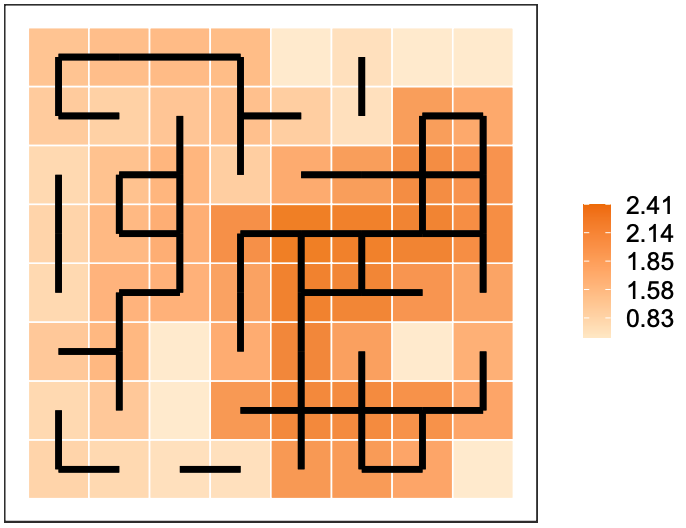
\includegraphics{images/square1.png}
    }}}
    \only<2>{  \makebox[\linewidth][c]{
    \resizebox{\linewidth}{!}{
      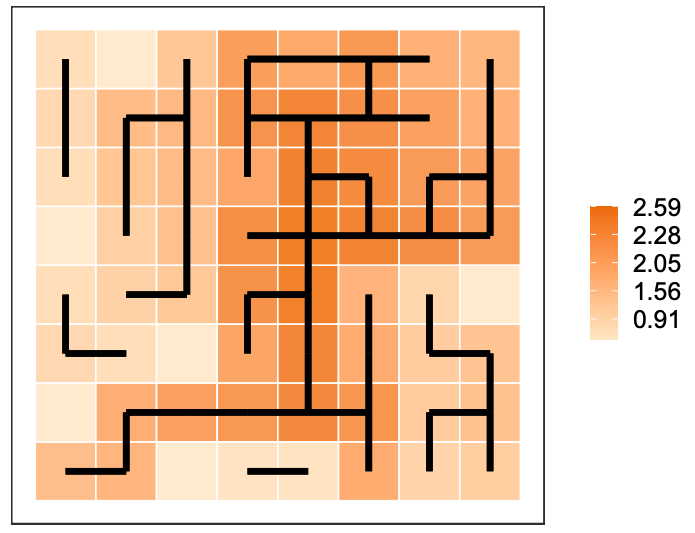
\includegraphics{images/square2.png}
    }}}
    \only<3>{  \makebox[\linewidth][c]{
    \resizebox{\linewidth}{!}{
      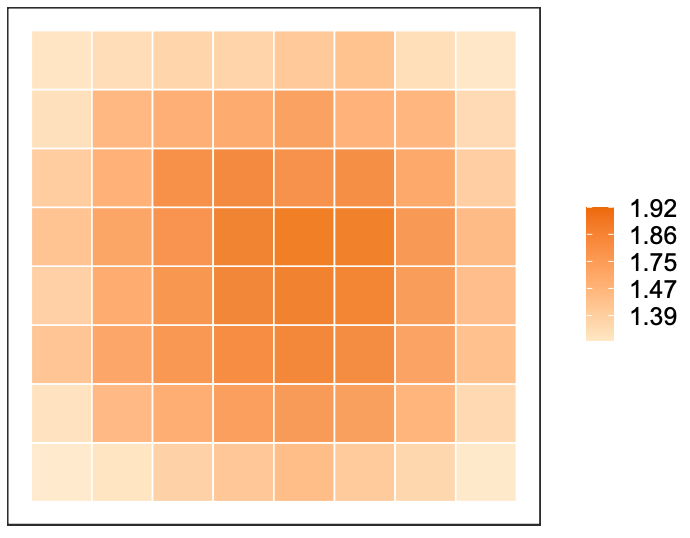
\includegraphics{images/square3.png}
    }}}
\end{column}%
\end{columns}
\end{frame}


\begin{frame}{ China: defining the counterfactual distribution}
\begin{columns}[T] % align columns
\begin{column}{.55\textwidth}
  \begin{wideitemize}
  \item In the stylized example, lines are laid randomly, making it easy to define the propensity scores
    \begin{itemize}
    \item What about in China?
    \end{itemize}
  \item What is the plausible counterfactual?
  \item<2-> Paper proposes an idea, and analagous to other examples
    \begin{itemize}
    \item Use \emph{planned} lines are randomized between unbuilt but planned, and built lines
    \item Calculate distribution of propensity score by constructing $MA_{i}$ under each counterfactual scenario
    \end{itemize}
  \end{wideitemize}
\end{column}%
\hfill%
\begin{column}{.45\textwidth}
    \only<1>{  \makebox[\linewidth][c]{
    \resizebox{\linewidth}{!}{
      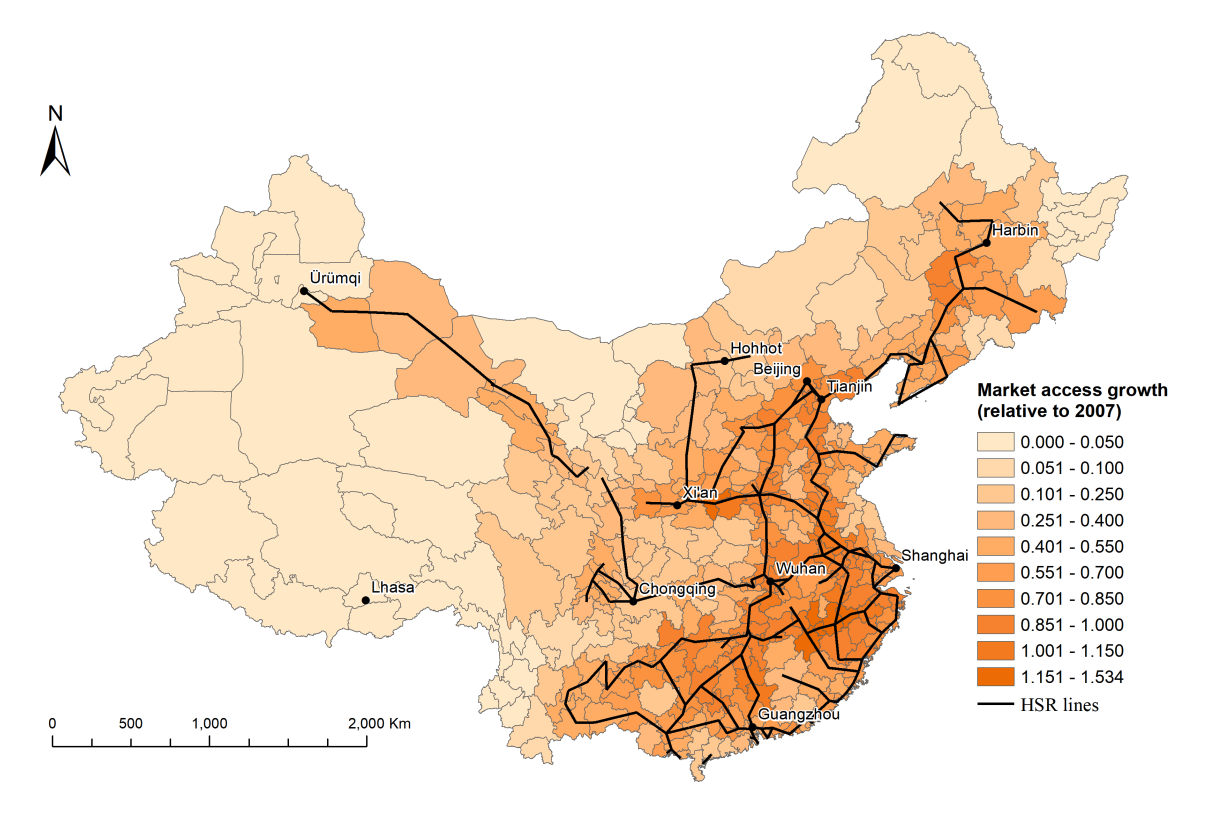
\includegraphics{images/china1.png}
    }}}
    \only<2>{  \makebox[\linewidth][c]{
    \resizebox{\linewidth}{!}{
      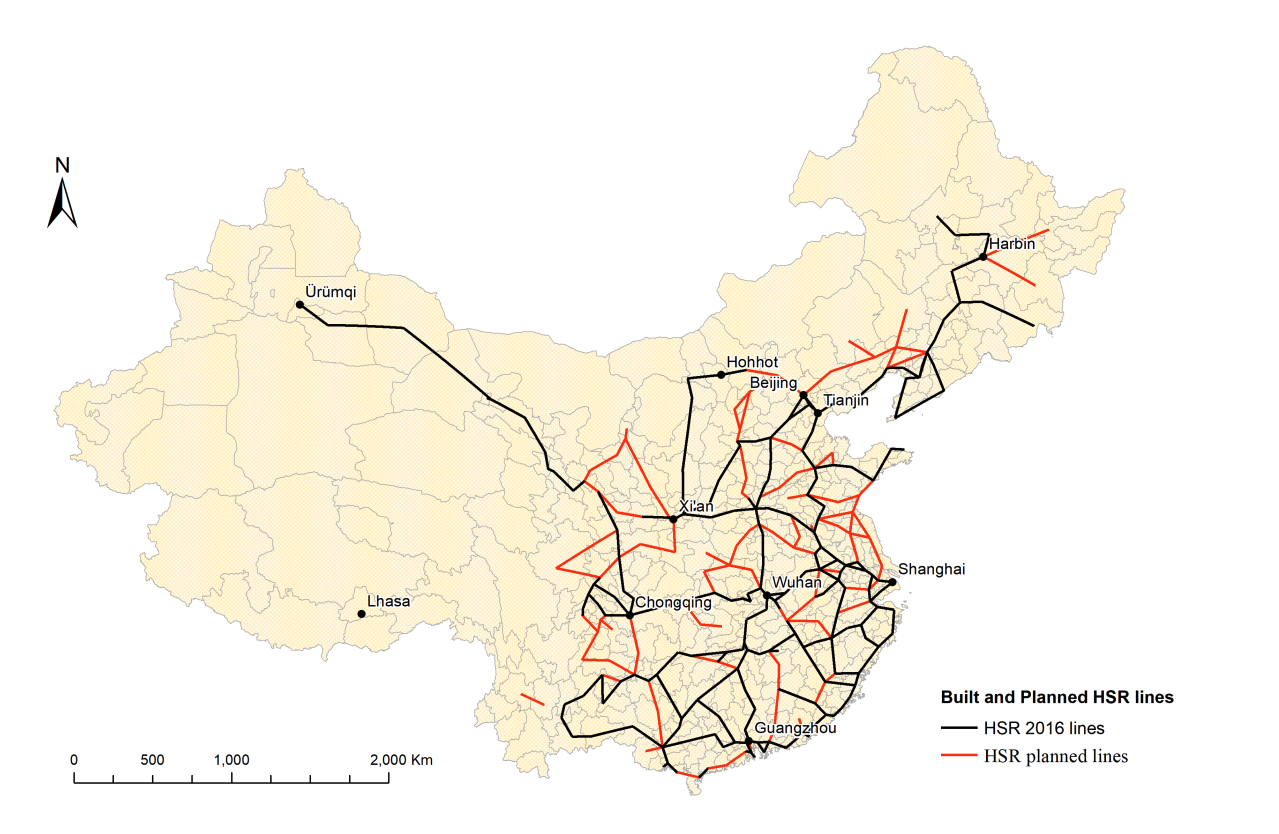
\includegraphics{images/china2.png}
    }}}
\end{column}%
\end{columns}
\end{frame}

\begin{frame}{China railroads: the punchline}
\begin{columns}[T] % align columns
\begin{column}{.25\textwidth}
  \begin{wideitemize}
  \item There was substantial bias from using OLS!
  \item Makes sense -- geography is king...
  \item No effect in randomized setting
  \end{wideitemize}
\end{column}%
\hfill%
\begin{column}{.8\textwidth}
    \makebox[\linewidth][c]{
    \resizebox{\linewidth}{!}{
      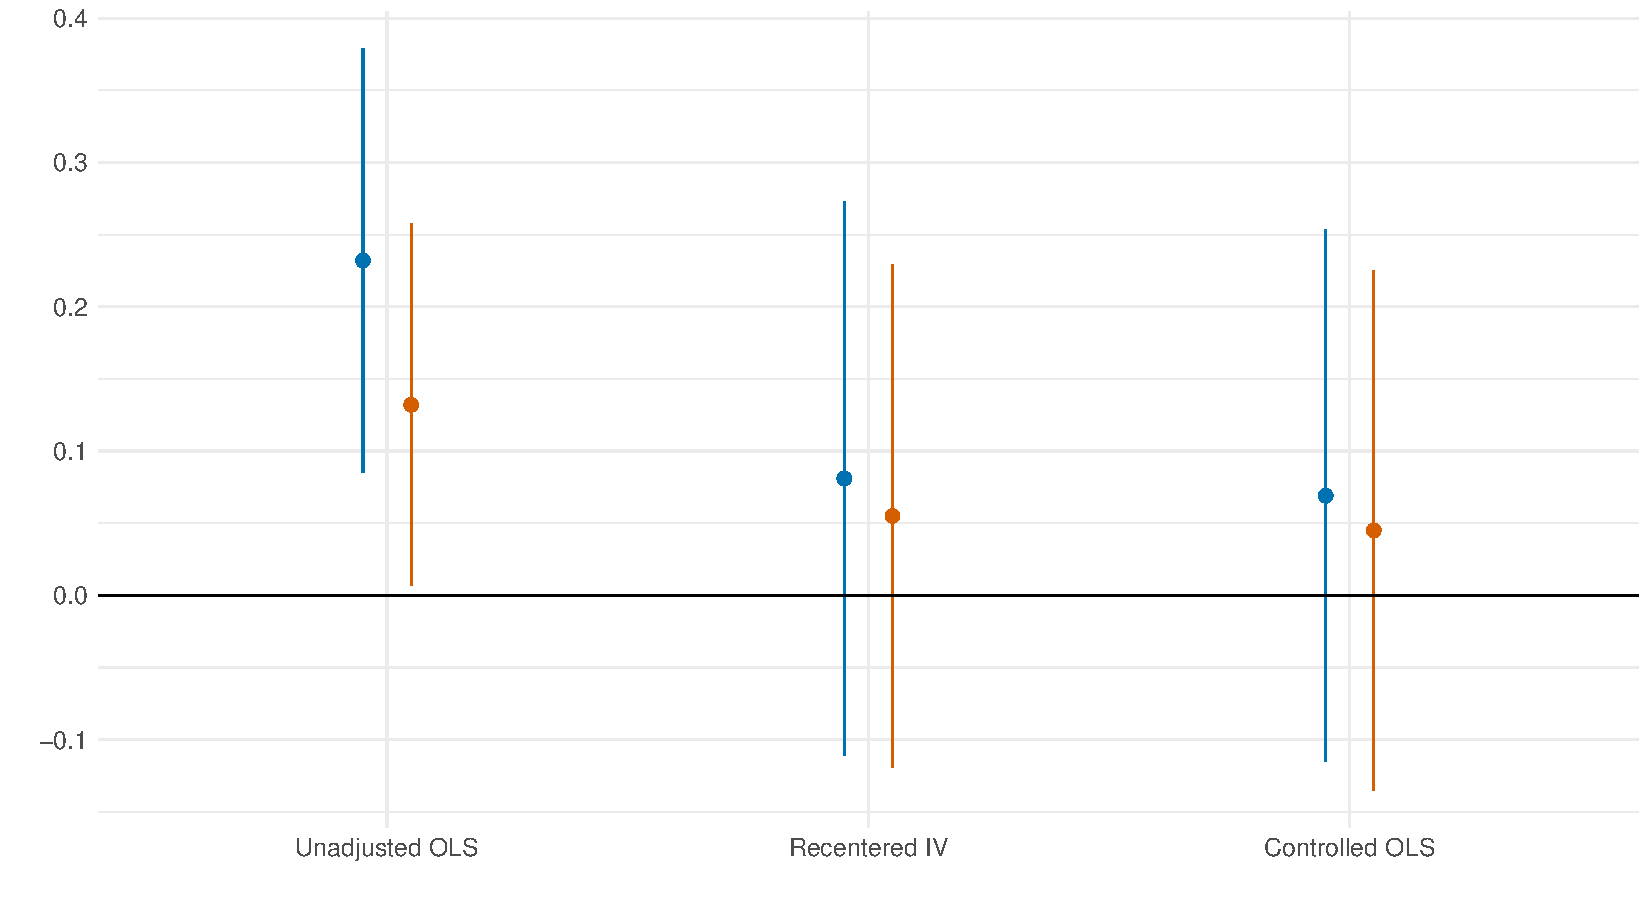
\includegraphics{images/china_estimates.pdf}
    }}
\end{column}%
\end{columns}
\end{frame}



\begin{frame}{ Defining the counterfactual distribution}
\begin{columns}[T] % align columns
\begin{column}{.9\textwidth}
  \begin{wideitemize}
  \item If one takes issue with the counterfactuals, that is
    reasonable (but of course, challenging to prove one way or the other)
  \item Key issue: this paper is just making \textbf{text} what was
    already \textbf{subtext}
    \begin{itemize}
    \item There was always an assumption about some counterfactual comparison in these designs!
    \end{itemize}
  \item The issue is that many of these paper do not understand how to describe the randomization aspect of their research design
    \begin{itemize}
    \item Consequentially, they cannot describe the ``as-if random''
      component coherently
    \item If a researcher has an alternative proposal, they should try that and see what estimates are available!
    \end{itemize}
  \item Also suggests that reserchers can show a ``range'' of
    estimates under different scenarios
  \end{wideitemize}
\end{column}%
\hfill%
\begin{column}{.45\textwidth}
    % \only<1>{  \makebox[\linewidth][c]{
    % \resizebox{\linewidth}{!}{
    %   \includegraphics{darts_map.jpeg}
    % }}}
\end{column}%
\end{columns}
\end{frame}


\begin{frame}{Key takeaways from paper}
  \begin{wideitemize}
  \item Provide a toolbox for contexts when economists have found good
    ``as-if'' random variation (and can describe the counterfactual
    distribution)
  \item Show that in cases where treatment is not influenced by
    others' treatment status, approach maps very tightly with
    traditional propensity methods, and can be much more efficient
  \item In spatial and network cases where treatment spillovers exist,
    show how to adjust for bias arising from units location on network
    or graph (or relevant characteristic)
  \end{wideitemize}
\end{frame}

\begin{frame}
\frametitle{Caveats}

\begin{wideitemize}
\item   We focused on Currie and Gruber (1996a, b) cases of simulated instruments, but there are other cases of ``simulated instruments'' 
\begin{itemize}
\item Gruber and Saez is all about characteristics (income) responding endogenously
\end{itemize}
\item These are tax elasticities and not clear that exclusion restriction holds
\item This tax literature is strongly tied to functional form or additional assumptions (see Blomquist, Newey, Kumar and Liang (2021))
\end{wideitemize}
\end{frame}

\begin{frame}{Granular Instruments (Gabaix and Koijen)}
\begin{columns}[T] % align columns
\begin{column}{.5\textwidth}
  \begin{wideitemize}
  \item Note that the previous approach heavily leaned on on
    considering a ``random'' distribution of exogeneous shocks,
    independent of the model
  \item Granular IV (Gabaix and Koijen (2022)) similarly relies on
    random shocks, but uses model structure to generate instruments
    for demand and supply estimation
  \end{wideitemize}
\end{column}%
\hfill%
\begin{column}{.5\textwidth}
  \makebox[\linewidth][c]{
    \resizebox{\linewidth}{!}{
      
\includegraphics{images/gabaix_koijen.png}
    }}
\end{column}%
\end{columns}
\end{frame}

\begin{frame}{Simplified Setup from Granular Instruments}
  \begin{wideitemize}
  \item Goal of the paper is to estimate a structural model of the following setup:
    \begin{align}
      y_{it} &= \phi^{d}p_{t} + \gamma^{y} X_{1,it} + \underbrace{\lambda_{i}\eta_{t}}_{\text{Unobserved}} + u_{it}\\
      p_{t}  &= \psi y_{St} + \gamma^{p} X_{2,t} + \epsilon_{t}\\
      y_{St} &= \sum_{i}\underbrace{S_{i}}_{\text{Size Weights}}y_{it}.
    \end{align}
  \item Effectively, we want to estimate the elasticities for this system:
  \end{wideitemize}
\end{frame}

\begin{frame}{ Setup from Granular Instruments}
  \begin{wideitemize}
  \item Goal of the paper is to estimate a structural model of the following setup:
    \begin{align}
      y_{it} &= \phi^{d}p_{t} + \gamma^{y} X_{1,it} + \underbrace{\lambda_{i}\eta_{t}}_{\text{Unobserved}} + u_{it}\\
      p_{t}  &= \psi y_{St} + \gamma^{p} X_{2,t} + \epsilon_{t}
    \end{align}
  \item A few things to note:
    \begin{enumerate}
    \item OLS is biased for either regression (can solve and show endogeneity bias)
    \item Equations are estimated in different aggregation levels (key!)
    \end{enumerate}
  \item Key assumptions for the paper:
    \begin{itemize}
    \item $u_{it}$ are completely random: $\boldsymbol{u}_{t} \perp \eta_{t},\gamma^{y} X_{1,it}, \gamma^{p} X_{2,t}$
    \item Models are correctly specified
    \end{itemize}
  \end{wideitemize}
\end{frame}

\begin{frame}{\emph{Simplified} Setup from Granular Instruments}
  \begin{wideitemize}
  \item Simplified application:
    \begin{align}
      y_{it} &= \phi^{d}p_{t} + \eta_{t} + u_{it}\\
      p_{t}  &= \psi y_{St} + \epsilon_{t}
    \end{align}
  \item Aggregate risk exposure is identical ($\eta_{t}$)
  \item What happens if aggregate $y_{it}$ within-time period?
    \begin{itemize}
    \item $y_{S t} = \sum_{i}S_{i}y_{it}$. Everything is
      identical across firms except $u_{it}$.
    \item Define $z_{t} = y_{S t} - y_{E t} = \sum_{i}S_{i}y_{it} - n^{-1}\sum_{i}y_{it} = u_{St} - u_{Et}$
    \item By assumption, $z_{t}$ is independent of $\epsilon_{t}$! 
    \item By assumption, $E(z_{t}\eta_{t}) = 0$  AND $E(z_{t}u_{Et}) = 0$      
    \end{itemize}
  \end{wideitemize}
\end{frame}

\begin{frame}{\emph{Simplified} Setup from Granular Instruments}
    \begin{align}
      y_{it} &= \phi^{d}p_{t} + \eta_{t} + u_{it}\\
      p_{t}  &= \psi y_{St} + \epsilon_{t}
    \end{align}
  
    \begin{wideitemize}
    \item Conceptually, this model has no external instruments, but if
      it is correctly specified, it can identify residuals which are
      assumed to be independent
    \item E.g. consider the reduced forms:
      \begin{align}
        y_{St} &=  (1-\phi^{d} \psi)  \phi^{d}  \epsilon_{t} + (1-\phi^{d} \psi)\eta_t + (1-\phi^{d} \psi)u_{St}\\
        p_t &= (1- \phi^{d}\psi)^{-1}\psi \eta_{t} + (1- \phi^{d}\psi)^{-1} \psi u_{St} + (1- \phi^{d}\psi)^{-1} \epsilon_{t}
      \end{align}
  \end{wideitemize}
\end{frame}
\begin{frame}{\emph{Simplified} Setup from Granular Instruments}
    \begin{align}
      y_{it} &= \phi^{d}p_{t} + \eta_{t} + X_{it}\delta + u_{it}\\
      p_{t}  &= \psi y_{St} + \epsilon_{t}
    \end{align}
  
    \begin{wideitemize}
    \item How can this break? What if there is a time-varying characteristic we do not control for?
    \item Then, $z_{t}$ will capture this size weighted component --
      if it's correlated with the average shocks on either side, that
      will be problematic.
  \end{wideitemize}
\end{frame}




\begin{frame}{Application for Granular Instruments (Gabaix and Koijen 2022b)}
\begin{columns}[T] % align columns
\begin{column}{.5\textwidth}
  \begin{wideitemize}
  \item Shocks to mutual fund flows as a source of variation in demand
  \end{wideitemize}
\end{column}%
\hfill%
\begin{column}{.5\textwidth}
\only<1>{  \makebox[\linewidth][c]{
    \resizebox{\linewidth}{!}{
      
\includegraphics{images/gabaix_koijen2.png}
    }}}
\only<2>{    \makebox[\linewidth][c]{
    \resizebox{\linewidth}{!}{
      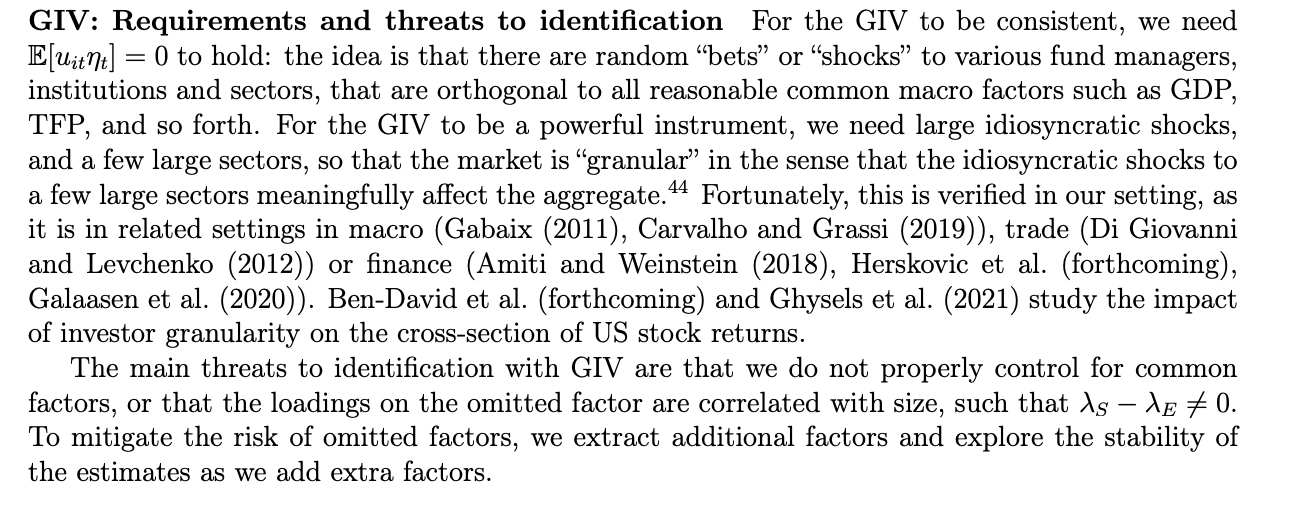
\includegraphics{images/gabaix_koijen3.png}
    }}}
\only<3>{    \makebox[\linewidth][c]{
    \resizebox{\linewidth}{!}{
      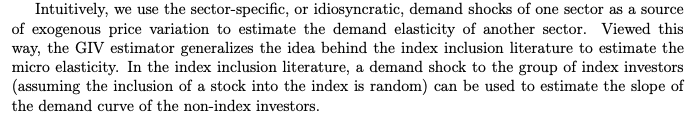
\includegraphics{images/gabaix_koijen4.png}
    }}}
\end{column}%
\end{columns}
\end{frame}


\end{document}
